%%%%%%%%%%%%%%%%%%%%%%%%%%%%%%%%%%%%%%%%%
% Beamer Presentation
% LaTeX Template
% Version 1.0 (10/11/12)
%
% This template has been downloaded from:
% http://www.LaTeXTemplates.com
%
% License:
% CC BY-NC-SA 3.0 (http://creativecommons.org/licenses/by-nc-sa/3.0/)
%
%%%%%%%%%%%%%%%%%%%%%%%%%%%%%%%%%%%%%%%%%

%----------------------------------------------------------------------------------------
%   PACKAGES AND THEMES
%----------------------------------------------------------------------------------------

\documentclass{beamer}

\mode<presentation> {

% The Beamer class comes with a number of default slide themes
% which change the colors and layouts of slides. Below this is a list
% of all the themes, uncomment each in turn to see what they look like.

%\usetheme{default}
%\usetheme{AnnArbor}
%\usetheme{Antibes}
%\usetheme{Bergen}
%\usetheme{Berkeley}
%\usetheme{Berlin}
%\usetheme{Boadilla}
%\usetheme{CambridgeUS}
%\usetheme{Copenhagen}
%\usetheme{Darmstadt}
%\usetheme{Dresden}
%\usetheme{Frankfurt}
%\usetheme{Goettingen}
%\usetheme{Hannover}
%\usetheme{Ilmenau}
%\usetheme{JuanLesPins}
%\usetheme{Luebeck}
\usetheme{Madrid}
%\usetheme{Malmoe}
%\usetheme{Marburg}
%\usetheme{Montpellier}
%\usetheme{PaloAlto}
%\usetheme{Pittsburgh}
%\usetheme{Rochester}
%\usetheme{Singapore}
%\usetheme{Szeged}
%\usetheme{Warsaw}

% As well as themes, the Beamer class has a number of color themes
% for any slide theme. Uncomment each of these in turn to see how it
% changes the colors of your current slide theme.

%\usecolortheme{albatross}
%\usecolortheme{beaver}
%\usecolortheme{beetle}
%\usecolortheme{crane}
%\usecolortheme{dolphin}
%\usecolortheme{dove}
%\usecolortheme{fly}
%\usecolortheme{lily}
%\usecolortheme{orchid}
%\usecolortheme{rose}
%\usecolortheme{seagull}
%\usecolortheme{seahorse}
%\usecolortheme{whale}
%\usecolortheme{wolverine}

%\setbeamertemplate{footline} % To remove the footer line in all slides uncomment this line
\setbeamertemplate{footline}[page number] % To replace the footer line in all slides with a simple slide count uncomment this line

\setbeamertemplate{navigation symbols}{} % To remove the navigation symbols from the bottom of all slides uncomment this line
}

\usepackage{graphicx} % Allows including images
\usepackage{booktabs} % Allows the use of \toprule, \midrule and \bottomrule in tables

%----------------------------------------------------------------------------------------
%   TITLE PAGE
%----------------------------------------------------------------------------------------

\title[Short title]{ELE 538B: ADMM in Neural Networks} % The short title appears at the bottom of every slide, the full title is only on the title page

\author{Zachary Hervieux-Moore} % Your name
\date{02/05/18} % Date, can be changed to a custom date

\begin{document}

\begin{frame}
\titlepage % Print the title page as the first slide
\end{frame}

\begin{frame}
\frametitle{Overview} % Table of contents slide, comment this block out to remove it
\tableofcontents % Throughout your presentation, if you choose to use \section{} and \subsection{} commands, these will automatically be printed on this slide as an overview of your presentation
\end{frame}

%----------------------------------------------------------------------------------------
%   PRESENTATION SLIDES
%----------------------------------------------------------------------------------------

%------------------------------------------------
\section{Review \& Problem Formulation} % Sections can be created in order to organize your presentation into discrete blocks, all sections and subsections are automatically printed in the table of contents as an overview of the talk
%------------------------------------------------

\subsection{Review} % A subsection can be created just before a set of slides with a common theme to further break down your presentation into chunks

\begin{frame}
\frametitle{Review}
\textbf{Neural Networks: }
  \begin{gather*}
    \min_{\theta} \mathcal{L}(f_\theta(x), y)
  \end{gather*}
  where $\mathcal{L}(\cdot)$ is some loss function and $f_\theta(\cdot)$ is a family of functions parameterized by your neural network, $x$ are the inputs, and $y$ are the outputs.

\textbf{ADMM: }
  Problems of the form
  \begin{gather*}
    \min f(x) + g(z) \\
    \text{s.t. } Ax + Bz = c
  \end{gather*}
  Can be solved using the following iterations
  \begin{gather*}
    x^{k+1} = \arg\min_x L_\rho (x, z^k, \lambda^k) \\
    z^{k+1} = \arg\min_z L_\rho (x^{k+1}) \\
    \lambda^{k+1} = \lambda^k + \rho (A x^{k+1} + B z^{k+1} - c)
  \end{gather*}

\end{frame}

%------------------------------------------------

\begin{frame}
\frametitle{Generative Adversarial Networks}
  Developed in 2014 by Goodfellow et al. Essentially, it is the combination of two different networks with opposing loss functions. The networks simultaneously minimize their loss which turns into the following minimax problem:
  \begin{gather*}
    \min_G \max_D = \mathbb{E}_{x \sim data} [\log D(x)] + \mathbb{E}_{z \sim p_z} [\log (1- D(G(z)))]
  \end{gather*}
  Where $D(x; \theta_d)$ is the discriminator network. It tries to minimize the error in the labels (real or generated). $G(z; \theta_g)$ is the generative network which takes in a noise vector $z$ and outputs something from your data space.
\end{frame}

%------------------------------------------------

\section{ADMM and Neural Networks}

\subsection{Toy Example}

\begin{frame}
\frametitle{Case Study 1: Toy Example}
  To motivate the potential usefulness of ADMM in neural networks, consider the following problem:
  \begin{gather*}
    \min_\theta \lVert f_\theta (x) - y \rVert_2^2 + \frac{1}{2} \lVert \theta \rVert_2^2
  \end{gather*}
  Turning this into ADMM
  \begin{gather*}
    \min_{\theta_1, \theta_2} \lVert f_{\theta_1} (x) - y\rVert_2^2 + \frac{1}{2} \lVert \theta_2 \rVert_2^2
  \end{gather*}
  Which yields
  \begin{gather*}
    \theta_1^{k+1} = \arg\min_{\theta_1} \lVert f_{\theta_1}(x) - y \rVert_2^2 + \langle \lambda^k, \theta_2^k - \theta_1 \rangle + \frac{\rho}{2} \lVert \theta_2^k - \theta_1 \rVert_2^2 \\
    \theta_2^{k+1} = \frac{\theta_1^{k+1} - \lambda^k}{1 + \rho} \\
    \lambda^{k+1} = \lambda^k + \rho (\theta_2^{k+1} - \theta_1^{k+1})
  \end{gather*}
\end{frame}

%------------------------------------------------

\begin{frame}
\frametitle{Case Study 1: Results}
  While the ADMM has more moving parts, it converges similarly to just doing SGD on the original problem

  \begin{figure}
    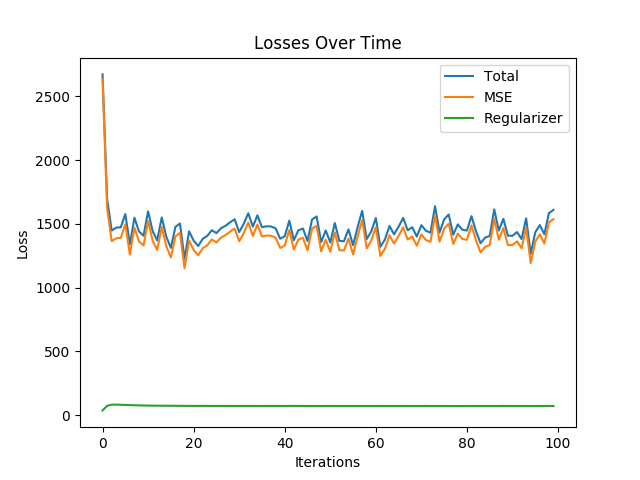
\includegraphics[width=0.4\linewidth]{./images/toy_loss.png}
    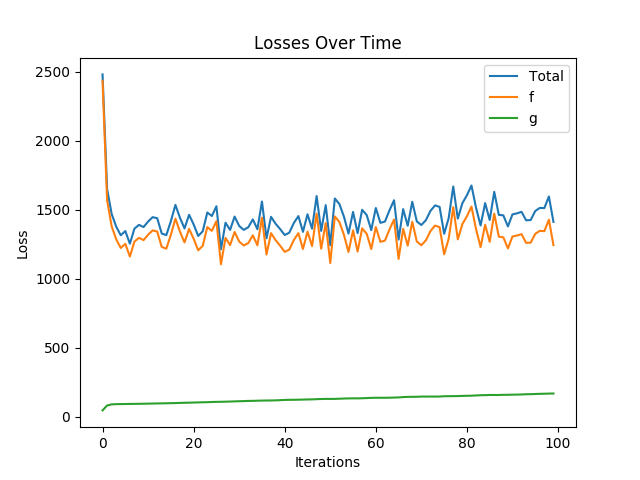
\includegraphics[width=0.4\linewidth]{./images/toy_admm_loss.png}
    \caption{Objective Value vs. Iterations for normal SGD on the left and ADMM on the right. Notice the slight slope for the loss associated with $g$ on the right.}
  \end{figure}
\end{frame}

%------------------------------------------------

\subsection{ADMM and GANs}

\begin{frame}
\frametitle{Case Study 2: GANs}
  Using the minimax formulation of GANs from before, we get the following problem for the discriminator
  \begin{gather*}
    \min_{\theta_d} \log D(x; \theta_d) + \log (1 - D(G(z); \theta_d))
  \end{gather*}
  Turning this into ADMM
  \begin{gather*}
    \min_{\theta_{d_1}, \theta_{d_2}} \log D(x; \theta_{d_1}) + \log (1 - D(G(z); \theta_{d_2}))
  \end{gather*}
  Which yields
  \begin{gather*}
    \theta_{d_1}^{k+1} = \arg\min_{\theta_{d_1}} \log D(x ; \theta_{d_1}) + \langle \lambda^k, \theta_{d_2}^k - \theta_{d_1} \rangle + \frac{\rho}{2} \lVert \theta_{d_2}^k - \theta_{d_1} \rVert_2^2 \\
    \theta_{d_2}^{k+1} = \arg\min_{\theta_{d_2}} \log(1 - D(G(z) ; \theta_{d_2})) + \langle \lambda^k, \theta_{d_2} - \theta_{d_1}^{k+1} \rangle + \frac{\rho}{2} \lVert \theta_{d_2} - \theta_{d_1}^{k+1} \rVert_2^2 \\
    \lambda^{k+1} = \lambda^k + \rho (\theta_{d_2}^{k+1} - \theta_{d_1}^{k+1})
  \end{gather*}
\end{frame}

%------------------------------------------------

\begin{frame}
\frametitle{Case Study 2: Results}
  While the ADMM implementation was actually faster per itertaion, below is the generative data from both models:

  \begin{figure}
    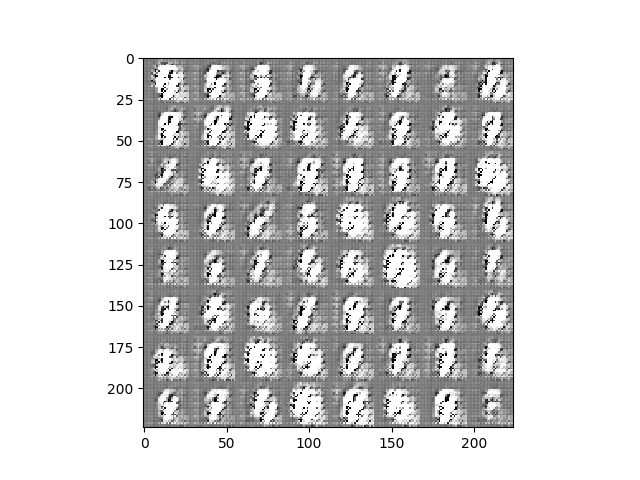
\includegraphics[width=0.2\linewidth]{./images/dcgan_50.png}
    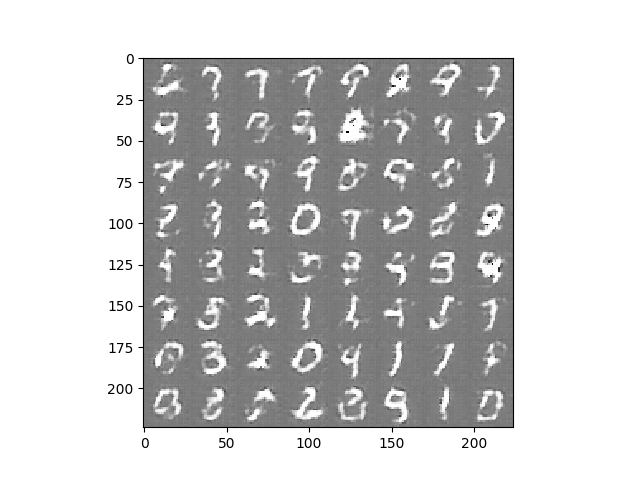
\includegraphics[width=0.2\linewidth]{./images/dcgan_150.png}
    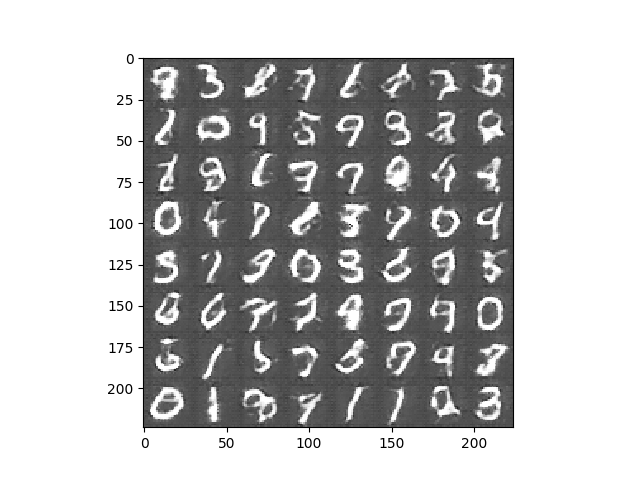
\includegraphics[width=0.2\linewidth]{./images/dcgan_250.png}
    \caption{Generative examples from the non ADMM model at the 50, 150, and 250 epochs.}
  \end{figure}

  \begin{figure}
    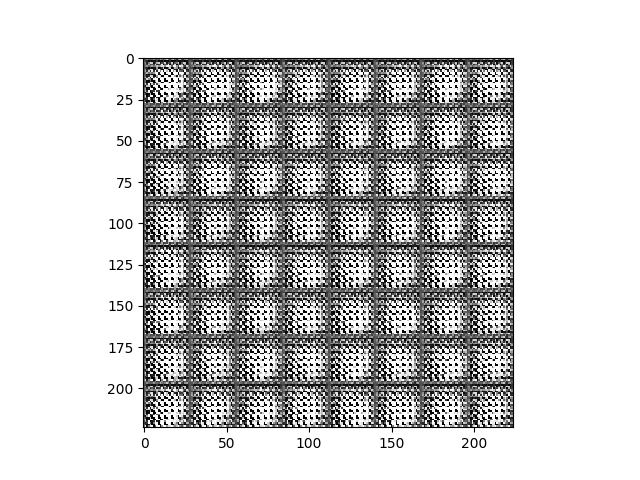
\includegraphics[width=0.2\linewidth]{./images/dcgan_admm_50.png}
    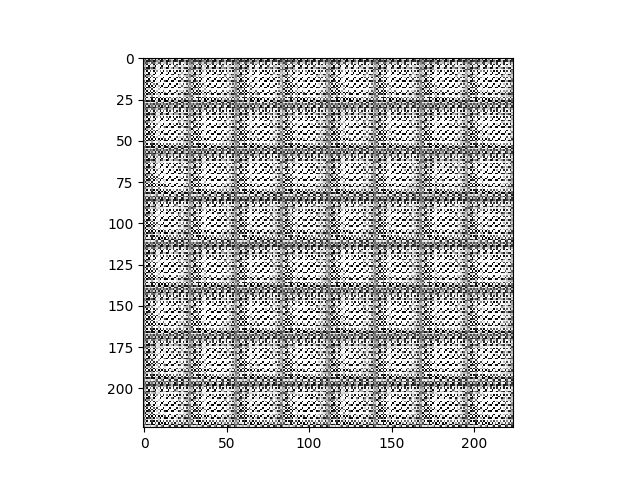
\includegraphics[width=0.2\linewidth]{./images/dcgan_admm_150.png}
    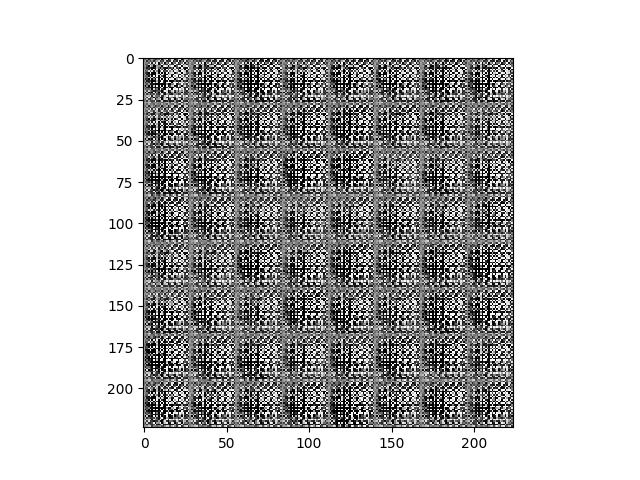
\includegraphics[width=0.2\linewidth]{./images/dcgan_admm_250.png}
    \caption{Generative examples from the ADMM model at the 50, 150, and 250 epochs.}
  \end{figure}
\end{frame}

%------------------------------------------------

\subsection{Problems and Possible Extensions}

\begin{frame}
\frametitle{Problems and Possible Extensions}
  The ADMM model was extremely sensitive to values of $\rho$ and implementation details.

  \begin{figure}
    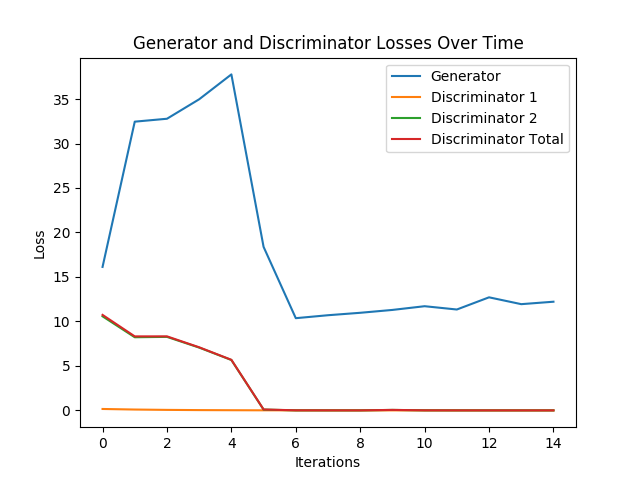
\includegraphics[width=0.4\linewidth]{./images/rho_loss_slow.png}
    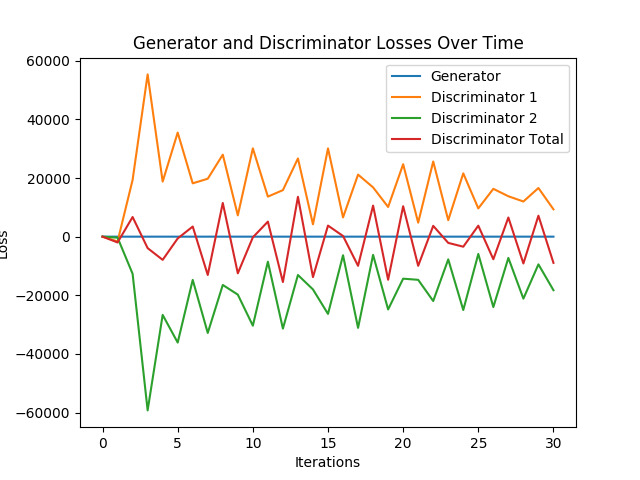
\includegraphics[width=0.4\linewidth]{./images/rho_loss_fast.png}
    \caption{Two experiments with the same $\rho$ value but with different implementations of the loss functions. The one on the right has floating point errors.}
  \end{figure}
\end{frame}

%------------------------------------------------

\begin{frame}
\frametitle{Possible Extensions}
  Possible extensions:
  \begin{itemize}
    \item Implementing some form of restart on the ADMM or only performing a few iterations of ADMM between normal SGD
    \item Modifying the objective function so that the two discriminators still have their objectives tied
    \item Enhancing the objective with many generators and discriminators and doing ADMM across those instead
  \end{itemize}
\end{frame}

%------------------------------------------------

%----------------------------------------------------------------------------------------

\end{document}